\documentclass[grado3]{LEMA-Tikz-IM}

\usepackage{graphicx}  % Needed to include graphics
\usepackage{pifont} % For the scissors symbol

\begin{document}
\begin{tikzpicture}
% \pgfplotsset{compat=1.18}

% page canvas letter size
\path (0,0) rectangle (8.5in,11in);

\def\myMargin{1in}

\coordinate (botLeft) at (\myMargin,\myMargin);
\coordinate (botRight) at (8.5in-\myMargin,\myMargin);
\coordinate (topRight) at (8.5in-\myMargin,11in-\myMargin);
\coordinate (topLeft) at (\myMargin,11in-\myMargin);

% clip outside the margin 
% \draw (botLeft) rectangle (topRight);


% find center of printable page
\coordinate (centerTop) at ($ (topLeft)!0.5!(topRight) $);

% add content
\node[anchor=north, text width=6.0in] (table) at ([yshift=-1in]centerTop) {%
    Este es otro rectángulo.

    \vspace{0.5cm}
    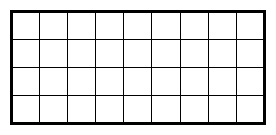
\includegraphics[scale=1.6]{../../svg-source/tikz-file-153048.pdf}
    \vspace{0.5cm}

    Podemos encontrar su área hallando $4 \times 9$.


    \begin{enumerate}
        \item Marca o colorea el rectángulo de una manera que te ayude a encontrar su área.
        \item Escribe una o más expresiones que representen lo que hiciste en el diagrama y muestra cómo encontraste el área.
    \end{enumerate}
};


% Add BLM heading to top and bottom
\node[below right, font=\bf\LARGE] (titulo) at (topLeft) {De diagramas a expresiones};
\node[font=\bf\large, below = 0.2ex of titulo.south west, anchor=north west] (subtitulo) {};


% Espacio de nombre
% \node[below left] at ([yshift=-6ex]topRight) {Nombre: \underline{\hspace{6cm}}};




\end{tikzpicture}
\end{document}